Given a embedded Giroux domain, this section describes a procedure
to remove its interior and "blow down" the resulting boundary.
We will refer to the procedure as "clean cut-out" of the Giroux domain.

These boundary components are always of the form $B = S^1 \times M$.
Topologically, blowing down is equivalent to simply gluing in $D^2 \times M$.

This operation can be performed in a way that respects the contact structure,
provided that $S^1 \times M$ has a neighborhood
of the form $[0, \epsilon)_s \times S^1_t \times M$ where $\alpha_M + s \d t$
defines a contact form.
In general this holds by \cite[Lemma 5.1]{MNW13} if the boundary components 
are $\xi$-round hypersurfaces, but it is also possible to show the existence 
of that neighborhood directly.

Let $D$ be the disk of radius $\epsilon$ in $\mathbb R^2$. The map 
\[
    \Psi \colon (re^{i\theta} , m) \mapsto (s = r^2, t = \theta, m)
\]
is a diffeomorphism from $(D \setminus \{0\}) \times M$ to 
$(0, \epsilon)_s \times S^1_t \times M$ s.t.
\[
    \Psi^*(\alpha_M + s \d t) = \Psi^*(\alpha_M) + \Psi^*(s\d t) 
    = \alpha_M + r^2 \d \theta,
\]
where the latter contact form can be extended to all of $D^2 \times M$.
In summary: If there is such a neighborhood of $M \times S^1$ as described above, 
we can glue $D \times M$ to $V \setminus B$ to get a new contact manifold 
in which $B$ has been replaced by $M$.

\begin{figure}
    \begin{subfigure}[t]{.293\linewidth}
        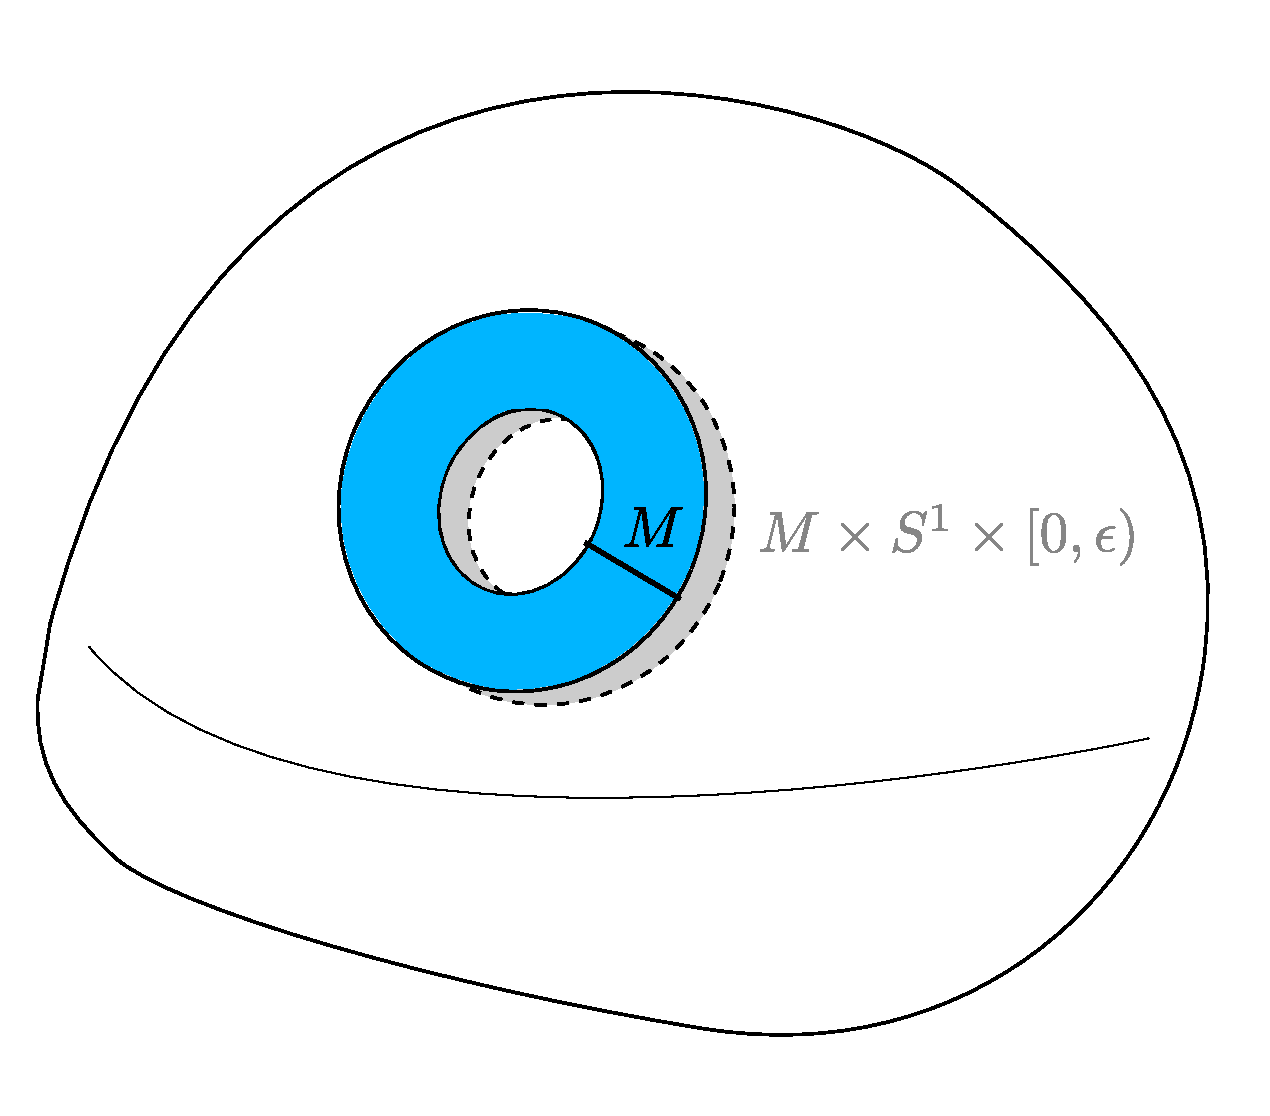
\includegraphics[width=\linewidth]{images/blow_down_before.pdf}
        \subcaption{The blue surface is a $\xi$-round boundary surface with (gray) neighborhood}
    \end{subfigure}\hspace*{.1\linewidth}
    \begin{subfigure}[t]{.6\linewidth}
        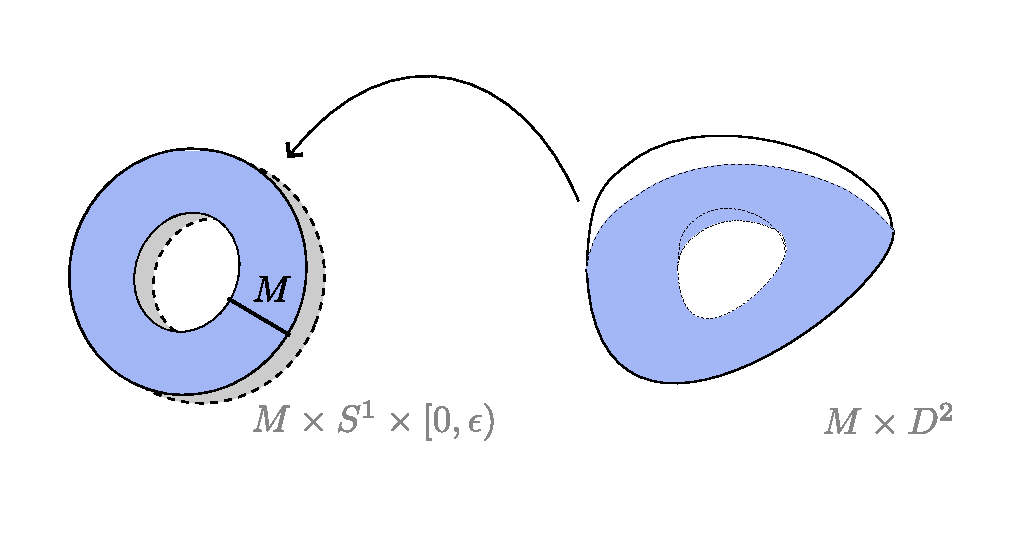
\includegraphics[width=\linewidth]{images/blow_down_topology.pdf}
        \subcaption{Topologically, the blowdown corresponds to gluing $M\times D^2$ 
        on top of the blue surface.}
    \end{subfigure}
    \begin{subfigure}{.9\linewidth}
        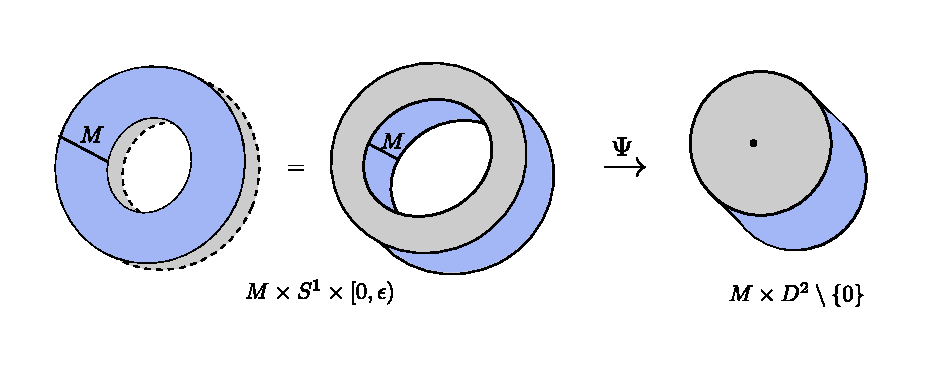
\includegraphics[width=\linewidth]{images/blow_down_contact.pdf}
        \subcaption{Visualization of $\Psi$: The neighborhood of the blue area
        $M \times S^1 \times \{0\}$ on the left is given by $M \times$ the gray annulus.
        In the middle, twist it so that the blue area sits on the inside.
        Applying $\Psi$ is simply retracting the inner circle of the gray annulus to a point.
        The blowdown effectively reduces the inner blue surface $M \times S^1$ to $M = M \times \{0\} \subset M \times D^2$.}
    \end{subfigure}
\end{figure}

Boundary components of Giroux domains are 
$\xi$-round hypersurfaces (\cite[Section 5.3]{MNW13}),
Therefore, after removal of a Giroux domain,
its boundary components can be blown down.
These two steps together form the clean cut-out.